\documentclass[10pt,a4paper]{article}
\usepackage[utf8]{inputenc}
\usepackage{amsmath}
\usepackage{amsfonts}
\usepackage{amssymb}
\usepackage{tikz}
\usepackage{graphicx}
\author{James Lee}
\title{6th Assignment of Computational Physics}
\begin{document}
	\maketitle
	\begin{abstract}
		In this report I present to you the numerical solution to Problem 2.9.
	\end{abstract}
	\section{Introduction}
	This program aims to compute the projectile motion.\\
	Projectile motion is governed by Newtonian mechanical laws. Therefore, it will not be difficult for us to solve projectile motion. However, one should take air drag effects into consideration if one wishes to find a rather accurate solution. In the following discussions, I will present to you numerical solutions with or without air drag.
	\subsection{Projectile Motion Without Air Drag}
	After a cannon is fired into vaccum gravitational field, its motion will only be influenced by gravity according to Newton's 2nd Law. It will be elementary for us to write down the ODE that describes the motion\\
	ODE to describe this model:
	\begin{equation}
	m\frac{d^{2}\vec{r}}{dt^{2}}=\vec{G}
	\end{equation}
	Component form:
	\begin{align}
	m\frac{d^{2}x}{dt^{2}}&=0\\
	m\frac{d^{2}y}{dt^{2}}&=-mg
	\end{align}
	with initial condition:
	\begin{align}
	x|_{t=0}&=0\\
	y|_{t=0}&=0\\
	v_x|_{t=0}&=v\cos{\theta}\\
	v_y|_{t=0}&=v\sin{\theta}
	\end{align}
	where $\theta$ is the firing angle.\\
	It is elementary for us to solve this set of ODE analytically:
	\begin{align}
	x&=v\cos{\theta}t\\
	y&=v\sin{\theta}t-\frac{1}{2}gt^{2}
	\end{align}
	The landing condition is $y=0$, therefore we have the landing moment to be $t=2v\sin{\theta}/g$, the firing range to be $\Delta x=v^{2}\sin{2\theta}/g$. Clearly, $\theta=45^\circ$ gives the maximum range.
	\subsection{Projectile Motion With Air Drag}
	When air drag is present, things are a little more complicated.\\
	The ODEs turn to:
	\begin{align}
	m\frac{d^{2}x}{dt^{2}}&=-B_{2}vv_{x}f(y)\\
	m\frac{d^{2}y}{dt^{2}}&=-mg-B_{2}vv_{y}f(y)
	\end{align}
    where:
    \begin{equation}
    f(y)=(1-\frac{ay}{T_0})^{\alpha}
    \end{equation}
    This set of ODE cannot be easily solved by analytical methods. The main contents of this reports devotes to numerical solution.
    \section{Main Content}
    \subsection{Air Drag Free Case}
    In order to determine the firing angle corresponding to maximum range, I write a program that can scan through different angle. (The Program is uploaded on my Github page).\\
    Apparently, the firing angle corresponding to maximum range is $\theta=45^\circ$.    
    The numerical solution to this case will be plotted in figure.1.
    \begin{figure}[htbp]
    	\centering
    	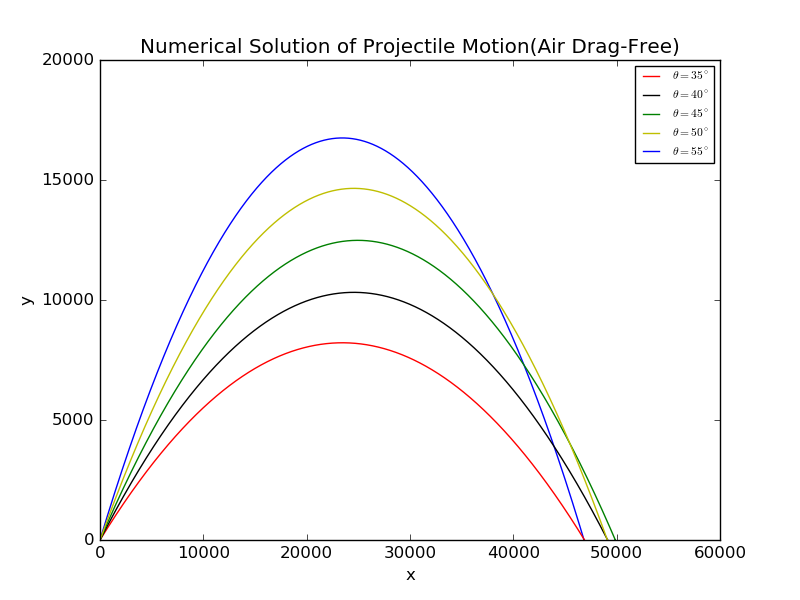
\includegraphics[width=5in]{Drag_Free.png}
    	\caption{Numerical Solutions with different $\theta$}
    \end{figure}
    
   \subsection{Air Drag Case}
   In order to solve the ODE numerically, we need to fix the parameters numerically.
   \begin{align}
   \frac{B_2}{m}&=4\times 10^{-5}\text{m}^{-1}\\
   a&=6.5\times 10^{-3}\text{ K}/\text{m}\\
   \alpha&=2.5\\
   T_{0}&=288\text{ K}
   \end{align}
   the initial conditions are:
   \begin{align}
   x|_{t=0}&=0\\
   y|_{t=0}&=0\\
   v_x|_{t=0}&=v\cos{\theta}\\
   v_y|_{t=0}&=v\sin{\theta}
   \end{align}
   where
   \begin{equation}
   v=700\text{ m}/\text{s}
   \end{equation}
   In order to determine the firing angle corresponding to maximum range, I write a program that can scan through different angle. (The Program is uploaded on my Github page).\\ 
   The program's results show that the firing angle corresponding to maximum range is
   \begin{equation}
   \theta=43.8^\circ
   \end{equation} 
   
    \begin{figure}[htbp]
    	\centering
    	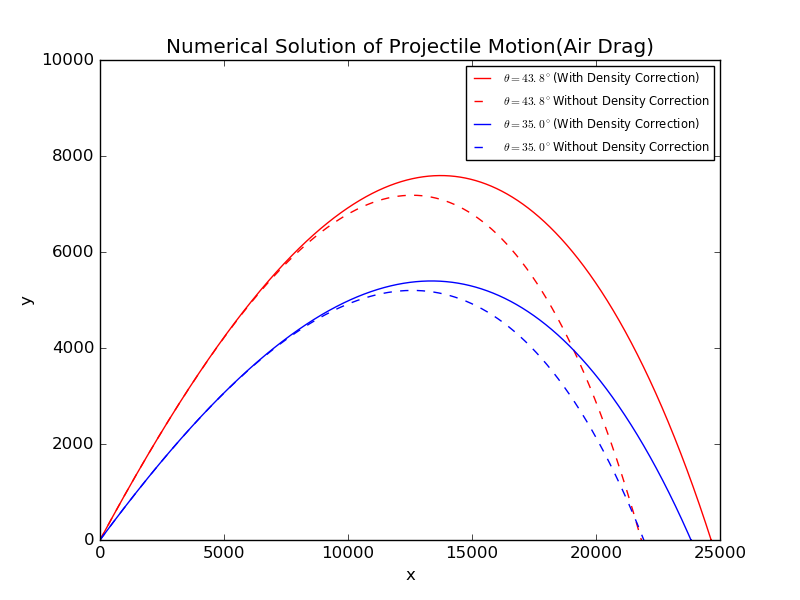
\includegraphics[width=5in]{Air_Drag.png}
    	\caption{Numerical Solutions\label{Figure_2}}
    \end{figure}
     The numerical solution to this case will be plotted in figure \ref{Figure_2}.
    As we can see in this figure, both solutions with or without density correction are presented. We can see clearly that by invoking density correction, the cannons are able to fly further in distance. This can be understood qualitatively: the density correction reduces the frictions on higher alititude, enabling the cannon to fly further in distance.
    
    \section*{Acknowledgement}
    When tackling this assignment, I benefitted a lot from the valuable discussions with Liu Xingchen. I would like to thank him for pointing out several syntax errors I made, also, for his willingness to discuss with me.
    
    \begin{thebibliography}{99}
    	\bibitem{}Hunter J, the Matplotlib Documentation, 2016
    	\bibitem{}Giordano N.J, Nakanishi H, Computational Physics, Pearson Education, 2007
    \end{thebibliography} 
\end{document}